\section{\textcolor{blue}{Deep Reinforcement Learning based Ensemble Model for Rumor Tracking}}
\label{sec:model}

\textcolor{blue}{RL-BRT model is inspired by Mixture of Experts model (MoE) \cite{DBLP:conf/nips/MillerU96}. MoE is an ensemble model that contains multiple separate sub-models. Each sub-model is an expert that is trained on a region of input data. The data distribution of each tweet is different and we believe each rumor tweet has its suitable classifier. Therefore, instead of dividing the input data into different regions, RL-ERT adopts a policy gradient based neural network to generate a weight for each sub-model and then aggregates them together. Besides, the weight changes according to each input sample.}

Ensemble model \cite{DBLP:journals/ml/Breiman96b} aggregates different basic models as its components. With a proper ensemble strategy, the performance is usually better than that of the basic models. Ensemble model reduces variance and improves the
stability of estimated density. Besides, the multiple components balance each other to reduce overfitting. Also, the most suitable classifier for different types of features is changing, and therefore multiple components are more likely to contain the proper classifier. Moreover, the importance of components changes according to the samples. Therefore, we propose a reinforcement learning based weight-tuning policy network (WTPN) to generate a suitable weight to balance the importance of components for each sample. 

\subsection{Architecture}
\label{sec:architecture}
The architecture of \textcolor{blue}{RL-ERT} is shown in Fig.~\ref{fig:architecture} . The input of \textcolor{blue}{RL-ERT} consists of two types of features, which include content features and social features. Then, all features are embedded and sent to basic components.  Some components such as TextCNN and BiLSTM use word-to-vector embeddings and the other components use particular embedding methods. Next, each trained component makes its prediction separately. Finally, we add the predicted results of all components and generate a final prediction by a reinforcement learning based ensemble algorithm.

\subsection{Preprocessing and Embedding}
\label{sec:process_embedding}
The textual content is one of the most important features in rumor tracking task. The length of the textual content is short, which is restricted within 140 words. Usually, the spelling in tweets is causal with symbols mixed in it. Consequently, we clean the content before inputting them into the model. The preprocessing in NLP is roughly immobilized, we only make some minor adjustments. In this work, we adopt splitting on tweets, and then remove the punctuation and special characters. Next, we turn all characters into lowercase. Finally, we adopt lemmatization on all words.

We find that the embedding strategies have a significant impact on the performance of \textcolor{blue}{RL-ERT}. Therefore, we try different embedding strategies to find the most proper one. There are three commonly used embedding strategies: pre-trained embedding, self-trained embedding, and random embedding. Pre-trained embedding is trained on large-scale corpus, and the most representative ones are GloVe \cite{DBLP:conf/emnlp/PenningtonSM14} and Google News embedding \cite{googlenews}. The self-train embedding is to train embedding on the current dataset. And the random embedding is to assign each word to a unique embedding randomly. In this work, we try all three embedding strategies and the detailed performance is introduced in Section \ref{sec:experiment}. By comparing them, we finally choose random embedding as the embedding strategy in \textcolor{blue}{RL-ERT}.

\begin{algorithm}[tbp]
	\caption{Ensemble Algorithm}
	\label{algorithm:RL-BRT}
	\LinesNumbered % show line numbers
	\KwIn{$K_y = \left\{y_F', y_T', y_B', y_N', y_S' \right\}$: outputs of all components;
		$x \in R^{l \times d}$: a processed sample;
		$WTPN$: weight-tuning policy network}
	\KwOut{$R$: predicted result of \textcolor{blue}{RL-ERT};}
	\textbf{Initialize:} Outputs of \textcolor{blue}{RL-ERT}: $y' = [0]*m$, $R = 0$ \;
	$W_y =  WTPN(x, K_y)$ \;
	\For{$i$ in $\{F,T,B,N,S\}$}{
		$y'+= w_i \cdot y_i'$;
	}
	
	$R = argmax(y')$
\end{algorithm}

\subsection{Procedure of \textcolor{blue}{RL-ERT}}
As shown in Fig.~\ref{fig:architecture}, we make preprocessing on \textbf{content features}. Despite some content features, the tweets contain plenty of \textbf{social features}. As introduced in Section \ref{sec:problem}, the tweet's branch or thread is unknown in advance. Consequently, we omit some features that contain external information about the branch or thread. Finally, we choose ``screen name", ``reply to screen name", and ``hashtag" as the social features in \textcolor{blue}{RL-ERT}. We treat the social features as words and add them to the tweets, then concatenate the content features and social features. All components are trained respectively until getting convergence. When predicting, each component outputs an $m-$dimensional vector $y'$ after the softmax layer. Each component in $y'$ indicates the probability of the content belongs to this category. 

With all components in \textcolor{blue}{RL-ERT} trained, we aggregate them and make a final prediction on the rumor tracking task. Generally, frequently used bagging methods include \textbf{joint training} and \textbf{respective training}. Joint training means all models have one shared loss function, and all parameters are updated together. When predicting, the ensemble model directly outputs the final prediction. Respective training means we train each component respectively. When predicting, each component makes its prediction result. In \textcolor{blue}{RL-ERT}, we choose the respective training. 

As all components are trained, results are aggregated by an ensemble algorithm. The ensemble details of \textcolor{blue}{RL-ERT} are shown in Algorithm~\ref{algorithm:RL-BRT}. We denote the predicted result of \textcolor{blue}{RL-ERT} as $R$. The inputs of Algorithm~\ref{algorithm:RL-BRT} are a sample $x$ and its predicted results of all components, which are denoted as $K_y = \left\{y_F', y_T', y_B', y_N', y_S' \right\}$. Each element in $K_y$ is an $m-$dimensional vector. Then, $x$ and $K_y$ is sent to WTPN and the output is a set of weights denoted as $W_y$ (Line 2). Each element $y_i'$ in $K_y$ is assigned with a weight in $W_y$. Next, we sum the predicted results in $K_y$ with weights (Line 4). Finally, the category with the maximum possibility is the predicted result of \textcolor{blue}{RL-ERT} (Line 6). 

\begin{figure}[tbp]
	\hspace{0ex}
	\vspace{0ex}
	\centering
	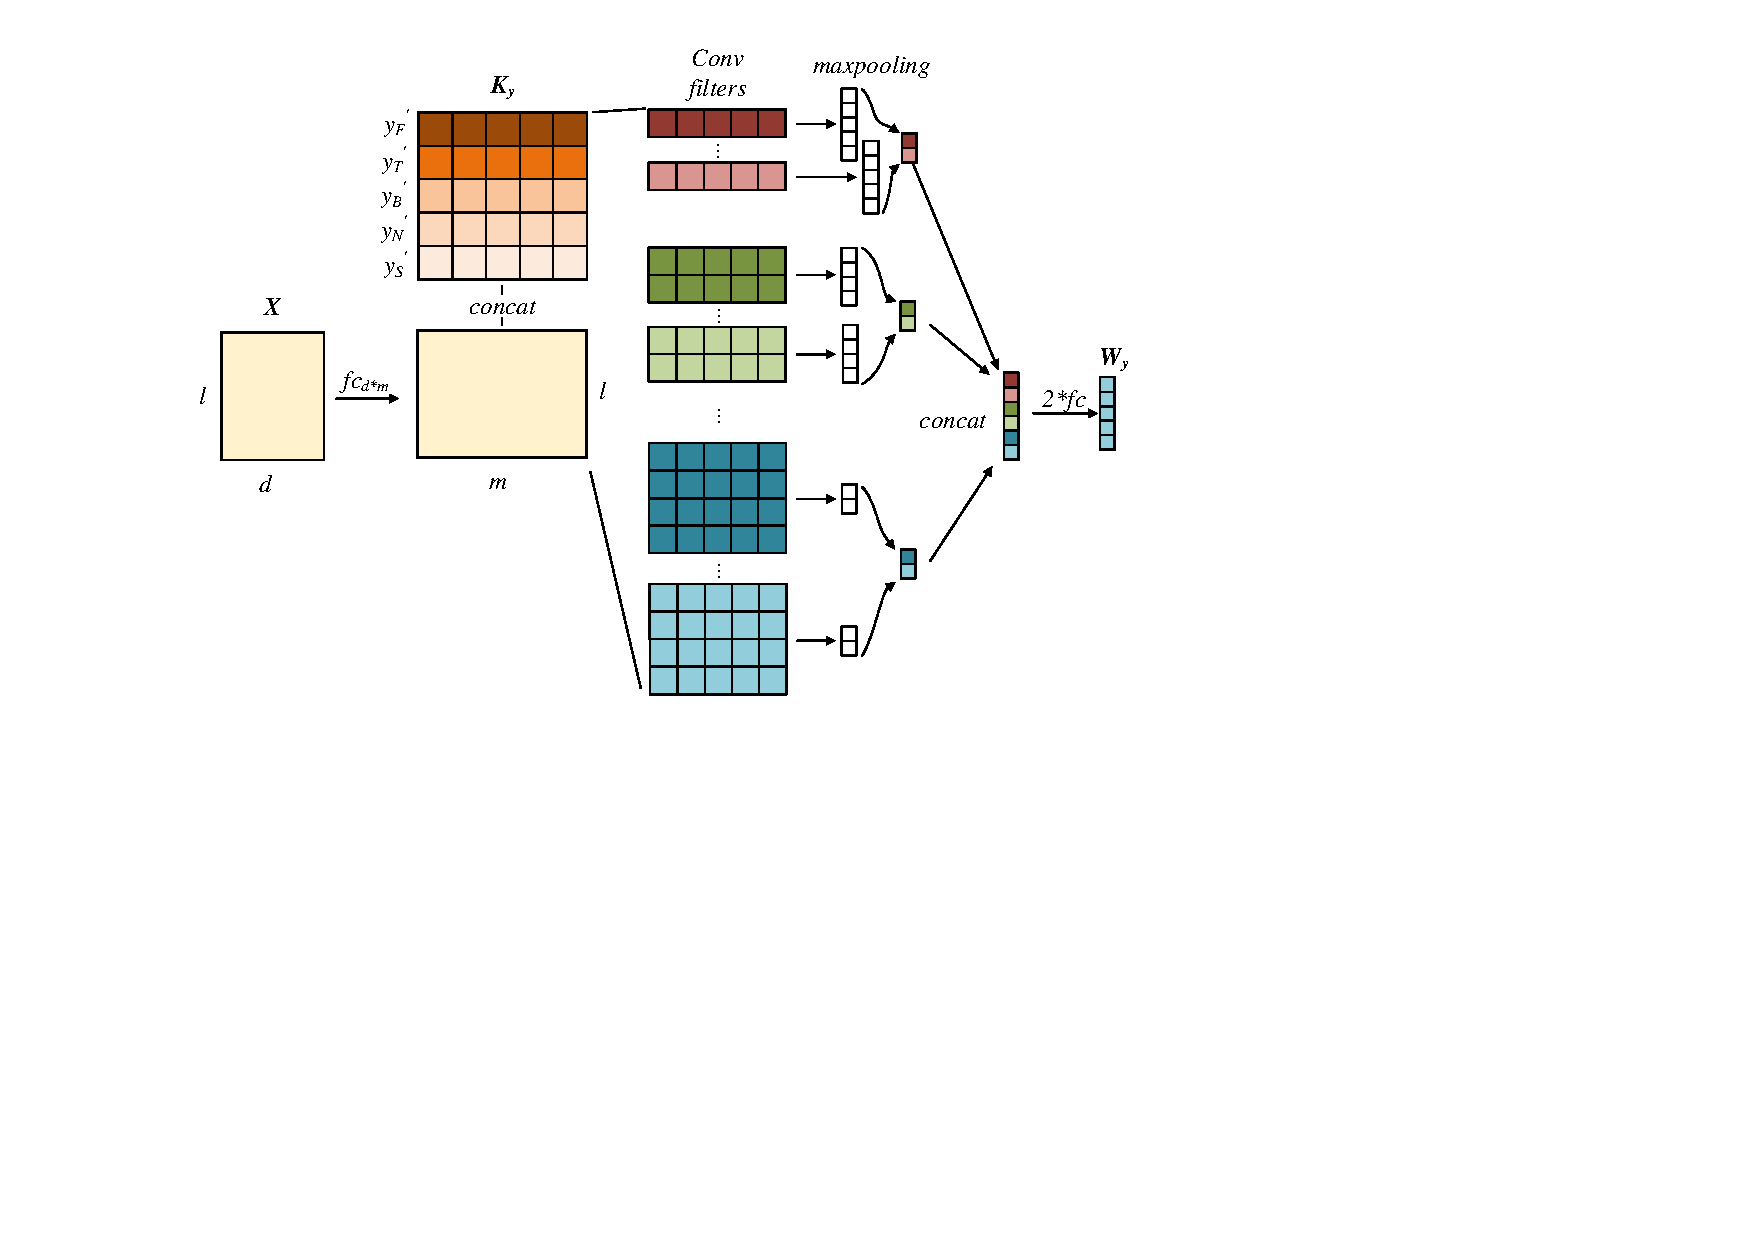
\includegraphics[width = \textwidth]{fig/WTPN}
	\caption{Structure of WTPN}
	\label{fig:WTPN}
\end{figure}

\subsection{Weight-Tuning Policy Network}
We propose WTPN to generate a suitable weight for each sample. WTPN is based on a reinforcement learning structure with a triple-tuple $<S, A, R>$, where $S = \{ s \}$ is a set of states. $A = \{ a \}$ is a set of actions. $R(s, a)$ is the reward function.
\begin{itemize}
	\item \textbf{State} $s$: $s = ( x, K_y )$ denotes a state of WTPN, where $x$ is a sample and $K_y$ is the set of classification results of $x$ generated by different classifiers.
	
	\item \textbf{Action} $a$: $a = W_y$ denotes a set of weights corresponding to elements in $K_y$.
	
	\item \textbf{Reward} $R$: $R(s, a) \to r \in R^{S * A}$ is a reward function that measures the profit of the current state-action tuple $(s, a)$.
\end{itemize}

For a batch of samples $X_b$, the accumulated reward is defined as:
\begin{equation}
R(s_1, a_1, ..., s_{|X_b|},a_{|X_b|}) = \frac{1}{|X_b|}\sum_{t = 1}^{t = |X_b|} r_t,
\end{equation}
where $ \frac{1}{|X_b|}$ is a normalization item. For a sample, $R(s,a) = r$ is the negative softmax cross-entropy loss between the predicted result (Line 6 in Algorithm \ref{algorithm:RL-BRT}) and ground-truth label.
For each batch, the parameter $\theta$ of policy function is updated by the following equation: 

\begin{align}
\theta &\leftarrow \theta + \lambda \nabla_\theta J_b(\mu_\theta),\\
J_b(\mu_\theta) &= \mathbb{E} [R(s_1, a_1, ..., s_{|X_b|},a_{|X_b|}) ],
\end{align}
where $\lambda$ is learning rate. $J_b(\mu_\theta)$ is the expected return.
The goal of WTPN is to approximate a policy function $\mu_\theta :S \to A$ that maximizes the accumulated reward.  Inspired by \cite{DBLP:conf/aaai/KimJSR16}, we propose a CNN based WTPN structure. As shown in Fig.~\ref{fig:WTPN}, the inputs of WTPN are $x$ and $K_y$, and the output is $W_y$. $x$ is sent to an FC (full-connect) layer and concatenated with $K_y$. We adopt multiple filters on the concatenated vector. The sizes of multiple filters are different, including  $[2*m]$, $[3*m]$, $[4*m]$, and $[5*m]$. The convolutional padding strategy is the same. By convolution and max-pooling, WTPN concatenates the captured features. Finally, with 2 FC layers, WTPN outputs $W_y$. \textcolor{blue}{In WTPN, we concatenate two separate inputs to a sequence. Then we use filters of different sizes to capture the features in different scales. Finally, we use max-pooling to reduce the model size and remove the unimportant parameters. The structure of WTPN is similar to TextCNN because TextCNN is an effective feature extractor, which is suitable to address the sequential data. Besides, the CNN based structure is calculated in parallel easily and is very efficient. Finally, we build a CNN based structure as shown in Fig.\ref{fig:WTPN}.}